\documentclass{beamer}
\mode<presentation>{\usetheme{Copenhagen}}

\usepackage[tikz]{bclogo}
\presetkeys{bclogo}{
	ombre=true,
	epBord=3,
	couleur = blue!15!white,
	couleurBord = red,
	arrondi = 0.2,
	logo=\bctrombone
}{}
\usepackage{etoolbox}
\makeatletter
\patchcmd{\insertverticalnavigation}%
{\ifx\beamer@nav@css\beamer@hidetext{\usebeamertemplate{section in sidebar}}\else{\usebeamertemplate{section in sidebar shaded}}\fi}%
{{\usebeamertemplate{section in sidebar}}}{}{}
\makeatother
\title{Machine Learning in Astronomy}
\author{Reza Monadi}
\institute{UC Riverside}
\date{May 14, 2020}
\begin{document}
	
	\frame{\titlepage}
	
	\begin{frame}
	\centering
	
\includegraphics[height=6cm, angle=0,origin=c]{ml.jpg}
	\tiny{credit: 365datascience.com}
	
\end{frame}

	
\section{Outline}
\frame{
	\begin{itemize}
		\uncover<1->{\item What is  \textbf{ML}?}
		\uncover<2->{\item How astronomy is tied to \textbf{BIG DATA}?}
		\uncover<3->{\item How to implement \textbf{ML} in astronomy? }
		\uncover<4->{\item How \textbf{ML} helps \textbf{SKA}?}
		\uncover<5->{\item What are the pitfalls of \textbf{ML} in astronomy?}
	\end{itemize}
	}

\section{ML overview}\frame{
		\centering
		
%\begin{figure}
	\centering
	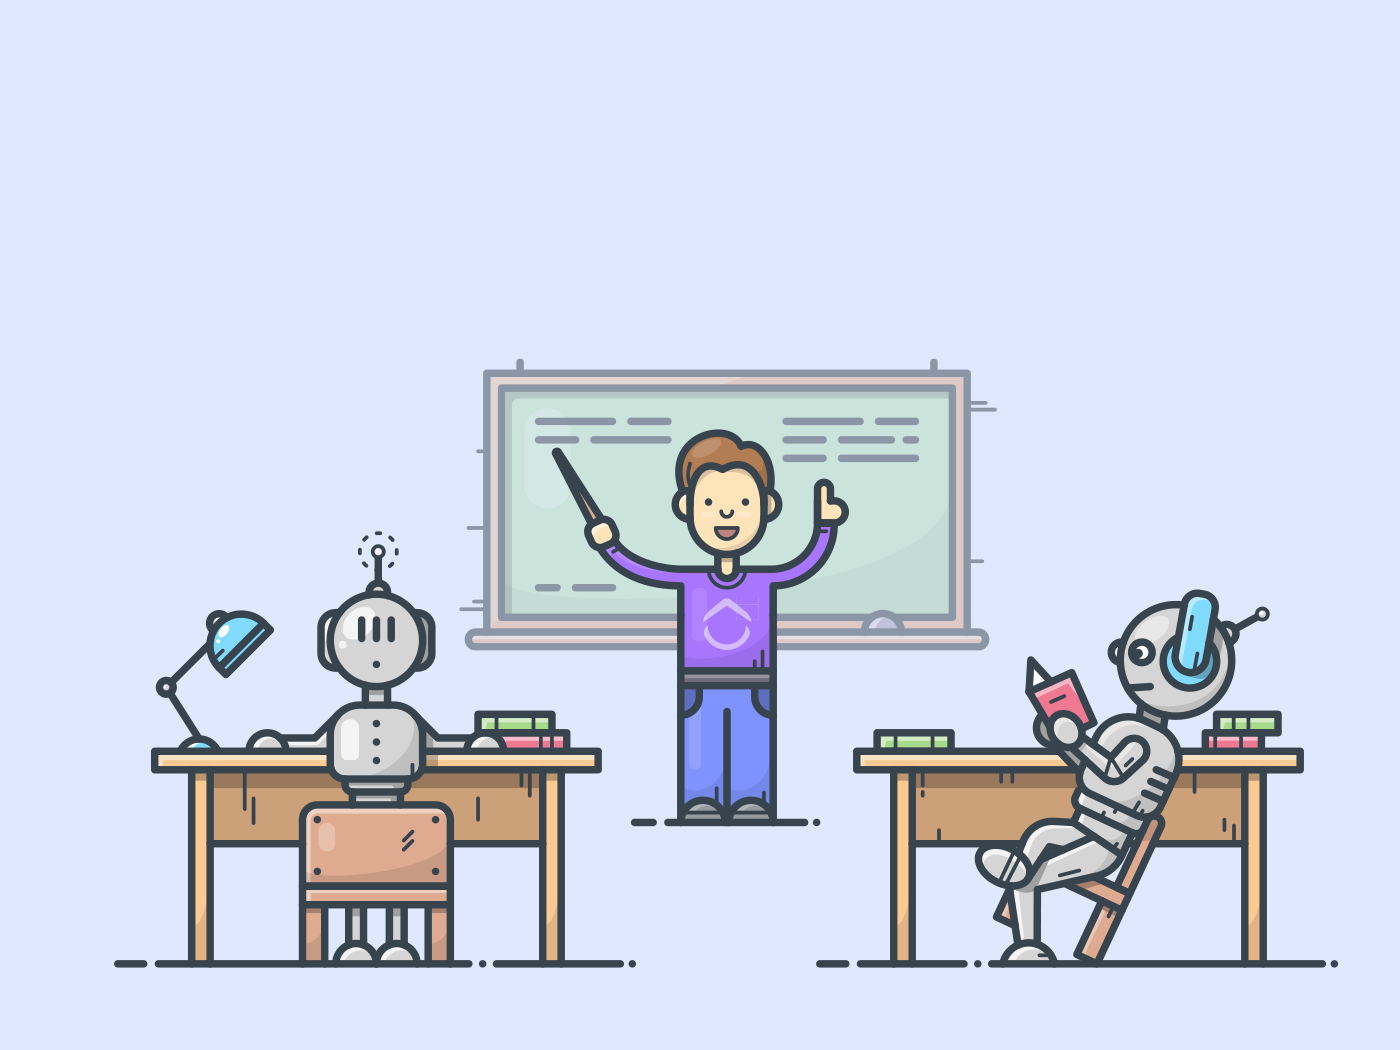
\includegraphics[width=0.8\linewidth]{external-content}
%	\caption{}
%	\label{fig:external-content}
%\end{figure}
%		{\tiny{credit: ClickUp (Productivity Platforms)}}
		}
	
\frame{
\begin{figure}
	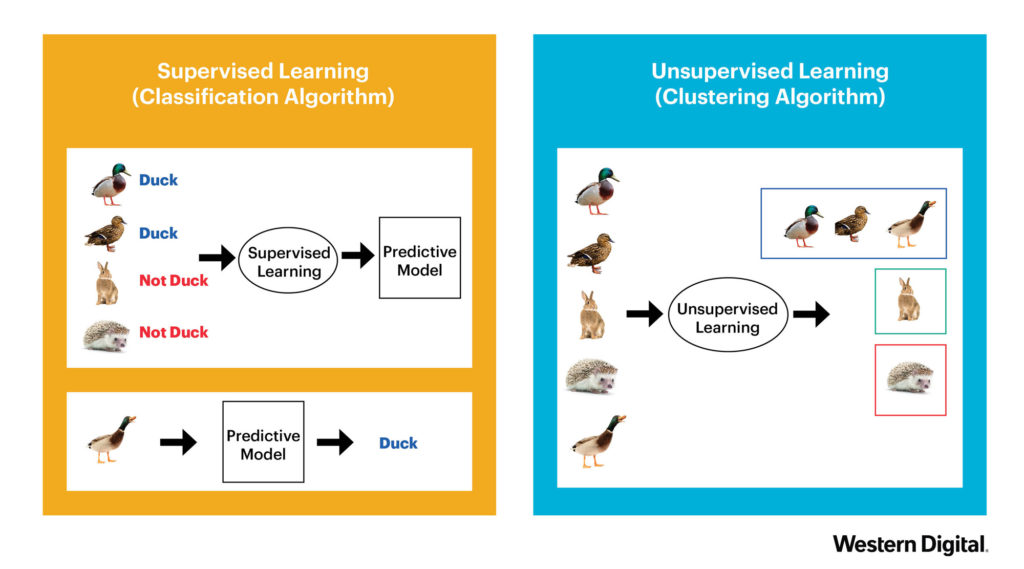
\includegraphics[width=\linewidth]{super.jpg}
%	\caption{}
%	\label{fig:example-supervised}
\end{figure}
}
\subsection{Supervised learning}
\frame{
	\frametitle{How supervised learning works?}
	\centering
	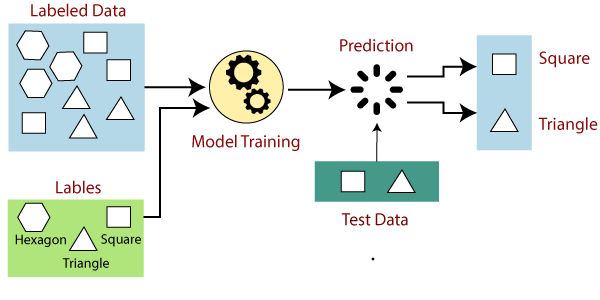
\includegraphics[width=\linewidth]{example-supervised.png}
	{\tiny{credit: javatpoint.com}}
	
}

\frame{\frametitle{Stages of Supervised Learning}
	
	\begin{itemize}
		\uncover<1->{\item Training: 
			\begin{enumerate}
				\uncover<2->{\item Select a model }
				\uncover<3->{\item Set up hyper-parameters of model}
				\uncover<4->{\item Teach the machine by training set}
		\end{enumerate} }
		\uncover<5->{\item Validation: 
			\begin{enumerate}
				\uncover<6->{\item Change the hyper-parameters  }
				\uncover<7->{\item Select the optimum hyper-parameters}
		\end{enumerate} } 
		\uncover<8->{\item Testing: 
			\begin{enumerate}
				\uncover<9->{\item Test learned model by an unseen part of the data-set. }
				\uncover<10->{\item Select the best model and use it for predictions.}
		\end{enumerate} } 
		
	\end{itemize}
}

\frame{ \frametitle{Supervised Learning vs Traditional Model Fitting ?}

\uncover<1->{\begin{bclogo}{Similarities}
		\begin{itemize}
			\uncover<2->{\item Both need a set of labeled measurements}
			\uncover<3->{\item Both need a model}
				
		\end{itemize} 
\end{bclogo}}	

\uncover<4->{\begin{bclogo}{Differences}
		\begin{itemize}
		\uncover<5->{\item Supervised learning: 
			\begin{enumerate}
				\uncover<6->{ \item The model gets adapted by data}
				\uncover<7->{\item Can be very nonlinear and complex}
				\uncover<8->{\item Designed for predicting unseen data}
			\end{enumerate}
					}
		\uncover<9->{\item Traditional model fitting: 
			\begin{enumerate}
				\uncover<10->{\item The model is predefined and has limited adaptivity}
				\uncover<11->{\item Useful for inferring relationships between  features}
			\end{enumerate}}
\end{itemize} \end{bclogo}}	
}

\subsection{Unsupervised learning}
\frame {\frametitle{How unsupervised learning works?}
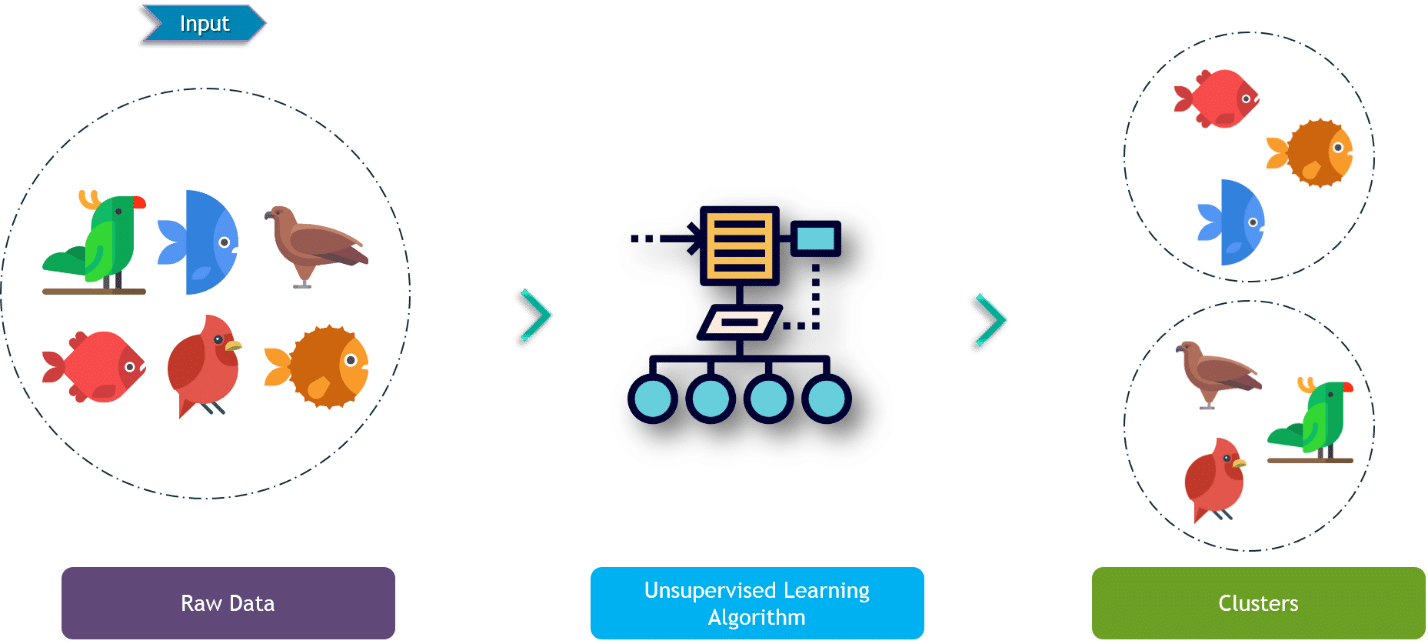
\includegraphics[width=\linewidth]{unsuper}
}
\frame{\frametitle{Clustering}
\begin{itemize}
	\uncover<1->{\item KMeans:}
	\uncover<2->{\item DBSCAN:}
	\uncover<3->{\item :}
	\uncover<4->{\item OPTICS:}

\end{itemize}
}
\section{Big Data in astronomy}
\subsection{Definition of BIG DATA}{
\frame{\frametitle{What is BIG DATA?}
\centering
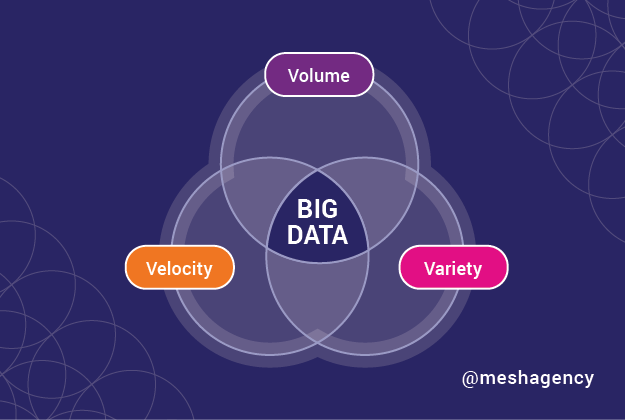
\includegraphics[height=6cm, angle=0,origin=c]{vvv.png}
}
\frame{\frametitle{VVV in astronomy}
\begin{itemize}
	\uncover<1->{\item Volume: larger quantities of data by better facilitates }
	\uncover<2->{\item Velocity: Higher speed of getting data }
	\uncover<3->{\item Verity: More complex structures of data }
\end{itemize}
}
%\subsection{Big telescopes}
%\frame{
%\frametitle{TMT}
%}
%\frame{
%	\frametitle{JWST}
%}
%\subsection{Higher resolution}\frame{}
%\subsection{Simulations}\frame{}
}
\subsection{Astronomical Surveys}
\frame{
	\frametitle{Sloan Digital Sky Server}
}
\frame{\frametitle{Large Synaptic Survey Telescope}}
\frame{
	\frametitle{Zwicky Transient Facility}
}

\frame{
	\frametitle{Gaia}
}
\frame{
	\frametitle{DESI}
}
\frame{
\frametitle{Square Kilometer Array}
}
\frame{\frametitle{\textcolor{red}{Astronomy} $\Rightarrow$ BIG DATA $\Rightarrow$ ML }
	
	
}

%\frame{\frametitle{BIG DATA and ML}
%	
%	%	\begin{columns}[c]
%	%		\column{.5\textwidth}
%	%		\begin{center}
%	%			\includegraphics[scale=0.3]{}
%	%		\end{center}
%	%		\column{.5\texwidth}
%	%		\begin{center}
%	%			\includegraphics[scale=0.3]{} 
%	%		\end{center}
%	%	\end{columns}
%	
%	
%	
\includegraphics[width=0.5\linewidth]{old-wise.jpeg}
%		
\includegraphics[width=0.45\linewidth]{clumsy.jpeg}
% }


\section{Supervised ML in astronomy}
\frame{
	\frametitle{List of Supervised learning algorithm used in astronomy?}
	
	\begin{itemize}
		\uncover<1->{\item Classification: discrete targets}
		\begin{enumerate}[a]
			\uncover<1->{\item Spectrum: quasar, star, galaxy, supernova, ...}
			\uncover<2->{\item Timing: Binary/isolated pulsar, variability,... }
			\uncover<3->{\item Galaxy morphology: spiral, dwarf, elliptical, ...  }
		\end{enumerate}
		\uncover<1->{\item Regression: continuous targets}
		\begin{enumerate}[a]
			\uncover<1->{\item }
			\uncover<2->{\item Photometry: redshift estimation }
			\uncover<3->{\item }
		\end{enumerate}
		
		\uncover<4->{\item DBSCAN:}
		\uncover<5->{\item :}
		\uncover<6->{\item OPTICS:}
		
	\end{itemize}
}
\subsection{Classification}\frame{}
\subsection{Regression}\frame{}
\subsection{Regression}\frame{}



\subsection{a}\frame{}
\subsection{b}\frame{}
\section{ML limitations}\frame{text}
\subsection{a}\frame{}
\subsection{b}\frame{}
\end{document}